\documentclass[11pt, a4paper]{article}
\usepackage{graphicx, fullpage, hyperref, listings}
\usepackage{appendix, pdfpages, color}
\usepackage{indentfirst} %段首空两格 棒
\usepackage{chngpage} 
\usepackage{tocloft}            % This squashes the Table of Contents a bit
\usepackage{pdfpages}
\usepackage{multirow}
\usepackage{amsmath}
\usepackage{amssymb}
\usepackage{framed}
%\usepackage{math}
%% Used on windows
%\usepackage[UTF8]{ctex}
%\usepackage{array}%需要该宏包

%% Used On Ubuntu
\usepackage{CJKutf8}


\setlength\cftbeforesecskip{3pt}
\renewcommand{\contentsname}{\centerline{\textbf{Content}}}
\graphicspath{{images/}}

\usepackage{multicol}

\usepackage{graphicx}
\usepackage{epstopdf}
\hypersetup{CJKbookmarks,%
	bookmarksnumbered,%
	colorlinks,%
	linkcolor=black,%
	citecolor=black,%
	plainpages=false,%
	pdfstartview=FitH}

%%%%%%%代码语法高亮设置

\usepackage{color}

\definecolor{pblue}{rgb}{0.13,0.13,1}
\definecolor{pgreen}{rgb}{0,0.5,0}
\definecolor{pred}{rgb}{0.9,0,0}
\definecolor{pgrey}{rgb}{0.46,0.45,0.48}

\usepackage{listings}
\lstset{
	language=Java,
	showspaces=false,
	showtabs=false,
	%%%%%
	frame = single,
	stepnumber = 2,  
	numbersep = 4pt, 
	 numbers=left,
	%breakatwhitespace=false, 
	tabsize=2,  
	%%%%%
	breaklines=true,
	showstringspaces=false,
    breakatwhitespace=false, 
	commentstyle=\color{pgreen},
	keywordstyle=\color{pblue},
	stringstyle=\color{pred},
	basicstyle=\ttfamily,
	%moredelim=[il][\textcolor{pgrey}]{$$},
	%moredelim=[is][\textcolor{pgrey}]{\%\%}{\%\%},
}


%%%%%%%%代码语法高亮设置

\definecolor{MyLightYellow}{cmyk}{0,0.,0.2,0} 

\setlength{\parskip}{4pt}        % sets spacing between paragraphs
\interfootnotelinepenalty=500    % this prevents footnotes breaking across pages


\title{
\includegraphics[width=0.45\textwidth]{dg}
        \\Facial Expression Summary   }          % <<<<<<<<< change the title as appropriate
\author{Jiaming Nie}                    % <<<<<<<<< module code

\begin{document}
\begin{titlepage}
	
%\date{\today}
\maketitle
\addtocontents{toc}{\protect\thispagestyle{empty}}
% because we don't want a page number on the title page
% Thanks to Huang Shanyue for suggesting this 

%\date{\today}
\thispagestyle{empty}  %去除首页页码
%\tableofcontents

\end{titlepage}

%\tableofcontents
%\listoffigures

%\newpage


\begin{CJK}{UTF8}{gbsn}

\section{选取网络以及相关参数}
网络的选取和相关参数可见如下表格

\begin{table}[htbp] 
	\begin{center}
		\caption{选取的网络和相关参数}
		\begin{tabular}{| l | l | l | l | l | l |}  \hline
	  Name & Batch Size & Epoch & Learning Rate & Optimizer & L2 Regularizer \\ \hline
	  ResNet18 & 16     & 10     & 0.1  &SGD & 0.0001\\ \hline
	  ResNet34 &  16   & 30   & 0.1  & SGD & 0.0001 \\ \hline
	  GoogleNet &  16 & 8  & 0.1  & SGD  & 0.0001 \\ \hline
		\end{tabular}
		
		\label{tab:kf_meaning2}
	\end{center}
\end{table}	

\section{训练结果与BaseLine}

\subsection{ResNet18}
对原有的ResNet 18网络添加了Batch Normalization层,在卷积添加了添加了Dropout层。

\subsubsection{ResNet18 准确率与损失曲线}

训练集和验证集的准确率(Accuracy)和损失(Loss)曲线可见图~\ref{fig:res18_loss},

\begin{figure}[htbp]
	\centering %使插入的图片居中显示
	
	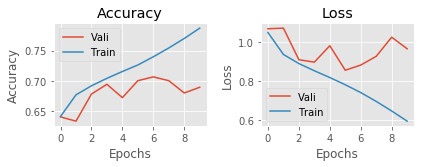
\includegraphics[width=10cm]{res18}
	\caption{ResNet 18 的准确率与损失曲线}
	\label{fig:res18_loss}
	%插入图片的标题,一般放在图片的下方,放在表格的上方
\end{figure}

\subsubsection{ResNet 18在测试集上的表现}

ResNet 18在测试集相关的结果如下:

\begin{table}[htbp] 
	\begin{center}
		\caption{ResNet18 在测试集的表现}
		\begin{tabular}{l | l}  \hline
			Accuracy  &  69.44\%  \\ \hline
			Recall        &  0.6944 \\ \hline
			F1 Score    & 0.6800 \\ \hline
		\end{tabular}
		\label{tab:res18_test}
	\end{center}
\end{table}	


\subsubsection{Confusion Matrix}

ResNet18在测试集上的Confusion Matrix 如下:

\begin{table}[htbp] 
	\begin{center}
		\caption{ResNet 18在测试集上的Confusion Matrix}
		\begin{tabular}{ | l | l | l | l | l |l | l |l | l | }  \hline
			&  Neutral  & Happy & Sad   &  Surprise   &  Fear  & Disgust  & Anger & Contempt  \\ \hline
			Neutral  & \textbf{0.7815}   & 0.1086  & 0.0298  & 0.0312  & 0.0081  &  0.0068  &  0.0326 & 0.0013 \\ \hline
			
			Happy   & 0.0922  & \textbf{0.8791}  & 0.0044   & 0.0111  & 0.0015   & 0.0037  & 0.0059  &  0.0014 \\ \hline
			
			Sad    & 0.4387 & 0.0592  & \textbf{0.3478}   & 0.0276  & 0.0276   & 0.0276  & 0.0711  & 	0  \\ \hline
			
			Surprise    & 0.4326   & 0.1063  &  0.0212   & \textbf{0.2978}   & 0.099  &  0.0014  & 0.02836  &  0 \\ \hline
			
			Fear     & 0.3538  & 0.0307  &  0.0923  & 0.1231  & \textbf{0.2769}   & 0.0461  & 0.0769 & 0 \\ \hline
			
			Disgust      &  0.2619  & 0.1190  & 0    & 0.0714  & 0   & \textbf{0.3809}  &  0.1667 & 0 \\ \hline
			
			Anger       & 0.4521   & 0.0459  & 0.0498   & 0.0496  & 0.0191   & 0.0498  & \textbf{0.3371} &  0 \\ \hline
			
			Contempt   & 0.4339  & 0.4339  &  0.0377  & 0.0188  & 0  & 0.0186 &  0.0377 & \textbf{0.0186} \\ \hline
		\end{tabular}
		\label{tab:res18_cm}
	\end{center}
\end{table}	




\subsection{ResNet 34}
对原有的ResNet 34网络添加了Batch Normalization层,在卷积添加了添加了Dropout层。

\subsubsection{ResNet34 准确率和损失曲线}
训练集和验证集的准确率(Accuracy)和损失(Loss)曲线可见图~\ref{fig:res34_loss},

\begin{figure}[htbp]
	\centering %使插入的图片居中显示
	
	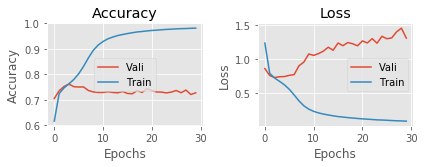
\includegraphics[width=10cm]{res34}
	\caption{ResNet 34 的准确率与损失曲线}
	\label{fig:res34_loss}
	%插入图片的标题,一般放在图片的下方,放在表格的上方
\end{figure}

在ResNet34的训练结果中,过拟合的程度超过GoogleNet和ResNet18,后两者在训练集上无法得到超过80\%的结果。

在最初几个Epoch以后验证集的准确率即趋于平稳。

\subsubsection{ResNet34 在测试集的表现结果}

ResNet34在测试集相关的数据如下:

\begin{table}[htbp] 
	\begin{center}
		\caption{ResNet34 在测试集的表现}
		\begin{tabular}{l | l}  \hline
			Accuracy  &  72.27\%  \\ \hline
			Recall        &  0.7227  \\ \hline
			F1 Score    & 0.7177  \\ \hline
		\end{tabular}
		\label{tab:res34_test}
	\end{center}
\end{table}	

\subsubsection{Confusion Matrix}
ResNet 34在测试集上Confusion Matrix如下:

\begin{table}[htbp] 
	\begin{center}
		\caption{ResNet 34在测试集上的Confusion Matrix}
		\begin{tabular}{ | l | l | l | l | l |l | l |l | l | }  \hline
			&  Neutral  & Happy & Sad   &  Surprise   &  Fear  & Disgust  & Anger & Contempt  \\ \hline
			Neutral  & \textbf{0.6807}   & 0.1426  & 0.0652  & 0.0353  & 0.0054 & 0.0013 &  0.0638 & 0.0054 \\ \hline
			
			Happy   & 0.0733  & \textbf{0.8873}  & 0.0074   & 0.011  & 0   & 0  & 0.0074  &  0.0007 \\ \hline
			
			Sad    & 0.225  & 0.059  & \textbf{0.577}   & 0.0237  & 0.0079   & 0.0079  & 0.0909  & 	0.0079  \\ \hline
			
			Surprise    & 0.2553   & 0.1276 & 0.0496   & \textbf{0.3972}   & 0.1134  &  0  & 0.0567 &  0 \\ \hline
			
			Fear     & 0.1846  & 0.0769 & 0.0461  & 0.1538  & \textbf{0.4615}   & 0  & 0.0769 & 0 \\ \hline
			
			Disgust      &  0.1428  & 0.0952  & 0.0476    & 0.0476  & 0.0238   & \textbf{0.3809}  &  0.2619 & 0 \\ \hline
			
			Anger       & 0.2452   & 0.0421  & 0.0689   & 0.0536  & 0.0191   & 0.0153  & \textbf{0.5517} &  0.0038 \\ \hline
			
			Contempt   & 0.3207  & 0.4905  &  0  & 0 & 0  & 0 &  0.0754 & \textbf{0.1132} \\ \hline
		\end{tabular}
		\label{tab:res34_cm}
	\end{center}
\end{table}	


\subsection{GoogleNet}

对原有的GoogleNet添加了Batch Normalization,L2正则化的系数设置为0.0001 (${10}^{-4}$)。

\subsubsection{GoogleNet 训练集与验证集准确率和损失曲线}
训练集和验证集的准确率(Accuracy)和损失(Loss)曲线可见图~\ref{fig:gn_loss},

\begin{figure}[htbp]
	\centering %使插入的图片居中显示
	
	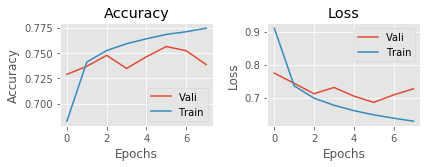
\includegraphics[width=10cm]{goonet}
	\caption{GoogleNet的准确率与损失曲线}
	\label{fig:gn_loss}
	%插入图片的标题,一般放在图片的下方,放在表格的上方
\end{figure}

在经历8个Epoch后,验证集的准确率为73.84\%,损失为0.727。训练集的准确率为77.44\%,损失为0.6289.

\subsubsection{GoogleNet在测试集的表现}

在模型训练结束后,GoogleNet在测试集的表现如下:

\begin{table}[htbp] 
	\begin{center}
		\caption{GoogleNet在测试集的表现}
		\begin{tabular}{l | l}  \hline
  	    Accuracy  &  75.96\%  \\ \hline
  	    Recall        &  0.7596 \\ \hline
  	    F1 Score    & 0.7465 \\ \hline
		\end{tabular}
		\label{tab:gooNet_test}
	\end{center}
\end{table}	

\subsubsection{测试集结果的Confusion Matrix}

GoogleNet在测试集表现结果的Confusion Matrix:

\begin{table}[htbp] 
	\begin{center}
		\caption{GoogleNet在测试集上的Confusion Matrix}
		\begin{tabular}{ | l | l | l | l | l |l | l |l | l | }  \hline
		&  Neutral  & Happy & Sad   &  Surprise   &  Fear  & Disgust  & Anger & Contempt  \\ \hline
	 Neutral  & \textbf{0.8059}   & 0.121  & 0.026  & 0.02  & 0 & 0.0013 &  0.0229 & 0.0013 \\ \hline
	 Happy   & 0.059  & \textbf{0.9186}  & 0.00295   & 0.011  & 0   & 0  & 0.0074  &  0.0007 \\ \hline
	 Sad    & 0.346  & 0.06  & \textbf{0.4489}   & 0.0039  & 0.0236   & 0.0157  & 0.094  & 	0  \\ \hline
	 Surprise    & 0.2535   & 0.1338  & 0.042   & \textbf{0.45}   & 0.0633   &  0.007  & 0.0492 &  0\\ \hline
	  Fear     & 0.1384  & 0.0769 & 0.0923  & 0.1077  & \textbf{0.4923}   & 0  & 0.0923 & 0 \\ \hline
	  Disgust      &  0.2142  & 0.1667  & 0.0476    & 0   & 0.023   & \textbf{0.3095}  &  0.2381 & 0 \\ \hline
	  Anger       & 0.3168   & 0.0343  & 0.0458   & 0.0267  & 0.0038   & 0.0190  & \textbf{0.5534} &  0 \\ \hline
	  Contempt   & 0.2264  & 0.6603  &  0  & 0 & 0  & 0 &  0.0377 & \textbf{0.0754} \\ \hline
		\end{tabular}
		\label{tab:gooNet_cm}
	\end{center}
\end{table}	

\subsection{AffectNet Paper给出的confusion matrix}

AffectNet给出了使用AlexNe训练结果给出的BaseLin以使用Microsoft Cognitive Service Emotion API预测得到的结果~\cite{ref:affnet}.


\subsubsection{使用标准的多分类Loss Function}
AffectNet Paper中所给出的confusion matrix可见于下图\ref{fig:bn_cm}.

\begin{figure}[htbp]
	\centering %使插入的图片居中显示
	
	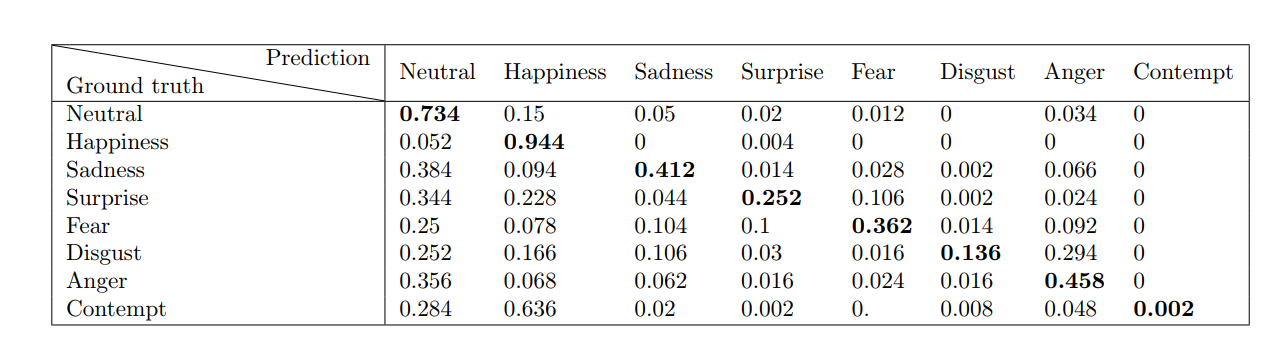
\includegraphics[width=16cm]{bn_cm}
	\caption{AffectNet Confusion Matrix}
	\label{fig:bn_cm}
	%插入图片的标题,一般放在图片的下方,放在表格的上方
\end{figure}

\subsubsection{使用加权损失函数}

AffectNet Paper中所给出的confusion matrix可见于下图\ref{fig:bn_cm}.

\begin{figure}[htbp]
	\centering %使插入的图片居中显示
	
	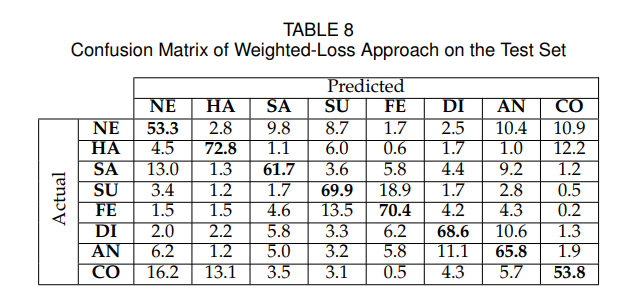
\includegraphics[width=16cm]{bn_cm2}
	\caption{AffectNet Confusion Matrix 使用加权损失函数}
	\label{fig:bn_cm2}
	%插入图片的标题,一般放在图片的下方,放在表格的上方
\end{figure}

加权损失函数提升了Sadness,Surprise, Fear, Disgust, Anger和Contempt的准确率,但所同时也降低了Neutral和Happy标签的准确率。

\subsubsection{AffectNet使用Microsoft Cognitive Service Emotion API}

微软表情API在识别Neutral和Happy标签的图片上给出了较高的准确率,但对一些负面情绪的标签识别准确较低在。

具体为:
\begin{itemize}
\item Neutral: 94\% (准确率过三种模型和BaseLine)
\item Happy:  85 \% 
\item Fear:  25 \%
\item Disgust: 27\%
\item Contempt: 4 \%
\end{itemize}

\section{一些API的调查}

\subsection{Microsoft Cognitive Services emotion API}

一家名为SightHound的公司对微软的情绪识别API进行了测试~\cite{ref:sight},表情的分为7种,总体准确率为61.3\%,Confusion matrix如下:

\begin{figure}[htbp]
	\centering %使插入的图片居中显示
	
	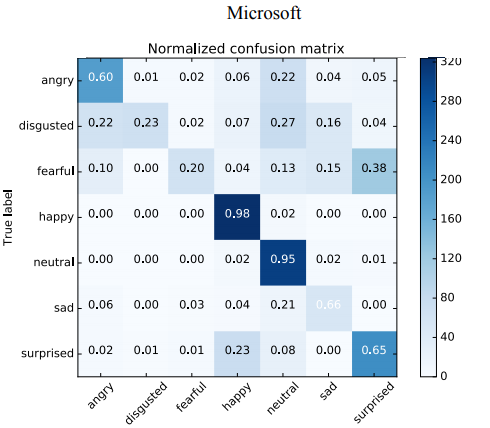
\includegraphics[width=12cm]{ms_cm}
	\caption{Sighthound使用MS API结果的 Confusion Matrix}
	\label{fig:ms_cm}
	%插入图片的标题,一般放在图片的下方,放在表格的上方
\end{figure}


\newpage

\subsubsection{EmotionNet}

EmotionNet Challenge~\cite{ref:emotionnet}是对一个包含95图片的数据库进行分类识别,2017年第一的队伍准确率为82\%.

\section{总结}

\subsection{网络深度问题}

对于AffectNet的表情数据集,使用了三种网络,ResNet18, ResNet34 和 GoogleNet, 在训练一个Epoch之基本验证集的效以及已经达到最好的效果,以上三种网络结构较复杂,可采取较为简单的网络模型。

\subsection{准确率问题}
三种模型共同特点是特点是对Neutral和Happ标签的准确率较高,可达到80\%和90\%左右,但是对其他标签准确率较低。基础的8类标签中,只有surprise这个标签可以是负面也可以是正面表情,其他表情可以分为Positive, Negative和Neutral标签。一些解决方案可如下:

\subsubsection{先分三类,再分8类}
可考虑先把标签分为正面(即Happy标签),中立(即Neutral) 以及负面(其余的5类)。训练时先将表情进行三分类,再对负面表情进行5分类。

\paragraph{混合标签}
仅Surprise表情而言,此标签在描述人表情的时一般和其它表情一同使用,可以考虑采用混合标签,比如惊讶且高兴,惊讶且难过等标注方式用于网络的训练。

\subsubsection{使用Arousal和Valence对表情进行回归}

Arousal表示情绪的正负面,Valence表示情绪的激烈程度,区间均为[-1,1]. AffectNe已经给出了所有图片相关的数值,可以使用神经网络解决这个回归问题。

\subsubsection{Action Unit 面部表情活动活动单元}

其他的数据集,如EmotionNet~\cite{ref:emotionnet},是标注表情的AU进而对表情进行分类。

EmotionNet~\cite{ref:en1}本身也给出了一种计算AU的方式。





\end{CJK}


%\tableofcontents

%\listoffigures
%\listoftables
%\lstlistoflistings        


%\newpage




\bibliographystyle{IEEEtran}  
\bibliography{MyRefs} 
\addcontentsline{toc}{section}{References}





%-------------------------------------------------------------------------------------------------------





\end{document}
